%% Chapter Template
%%\graphicspath{{/img}}
\chapter{Animation for Data Joins} \label{c3} % Main chapter title

\section{The logic of joins}

Joins allows us to combine the information in different data sets. This could be because we just want to keep all the data together instead of having multiple different sets of data stored separately. 

Another reason could be because we have multiple data sets which are related to each other and we would want to combine them together into a single data frame so we can perform statistical analysis on them.  Most analysis functions in \textsf{R} take data from a single data frame.

In a sense joins are just trying to combine data sets together based on some conditions, we can think of this as adding more columns or variables to one data set with the new information taken from the other data sets. These conditions are like some sort of instructions we give to the join, so it can output a data set that we desire. In joins, these conditions are defined by the key column, this is discussed in more detail in the next section. \\

All examples in the following section will be based on  the two toy data files shown in Fig.~\ref{fig:datoy1}.

\begin{figure}[H]
    % \centering
    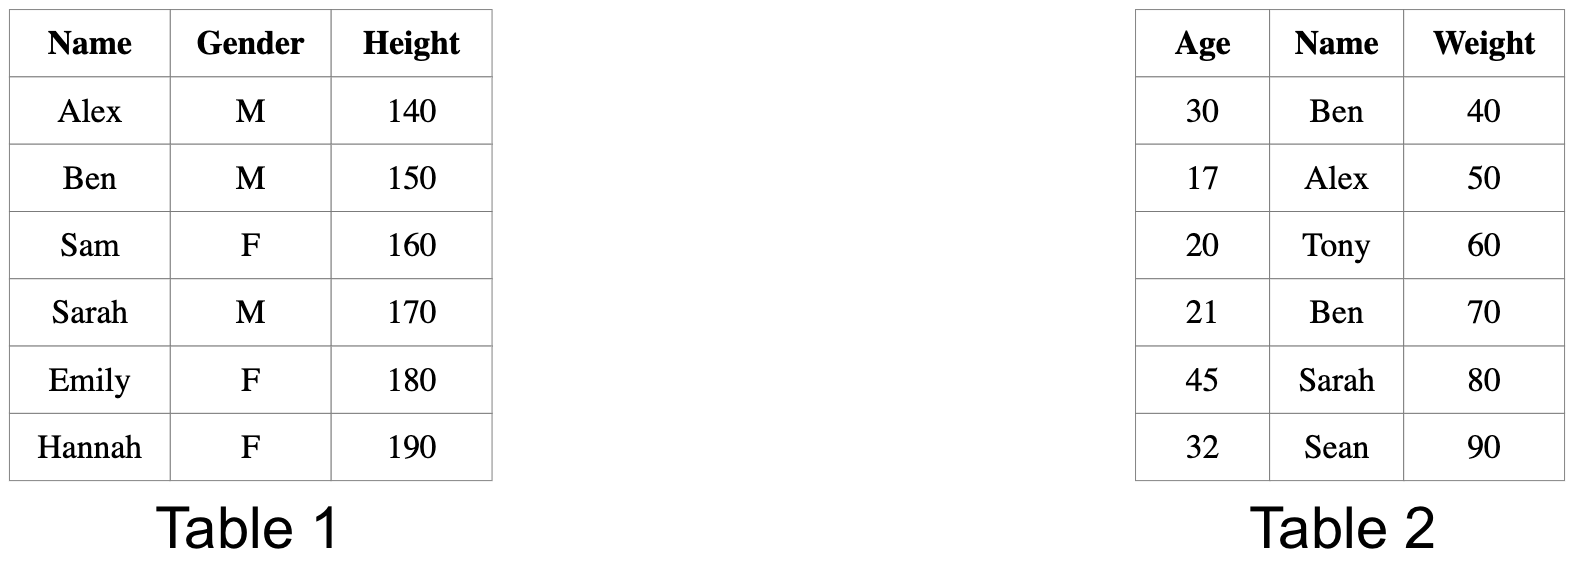
\includegraphics[scale = 0.25]{Masters-Thesis/img/datoy1.png}
    \caption{Toy data set}
    \label{fig:datoy1}
\end{figure}


\section{Linking key columns}

The problem we are trying to solve here is that we want to join the two tables together, to do this we will need to use the key column which is explained above. It gives us information on how the rows from the two tables are joined together. Without the key columns there will be no ways to define what rows belong together. In this section we will be discussing how to draw attention of the user to the key columns and their role. 

Initially, we want the user to focus on the key columns. We do this by first fading out the non-key columns. We use this fading strategy often when we want the user to focus on particular elements at that moment. Second, we show a line linking the key column from both tables. Third, we display a set of words stating which columns we are joining by.


\begin{figure}[H]
    % \centering
    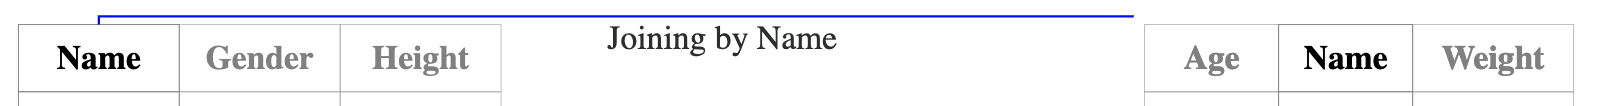
\includegraphics[scale = 0.25]{Masters-Thesis/img/keycol1.png}
    \caption{Key column step 1}
    \label{fig:keycol1}
\end{figure}

Forth, we flash the key column headers on both tables to further focus attention on the key columns.

\begin{figure}[H]
    % \centering
    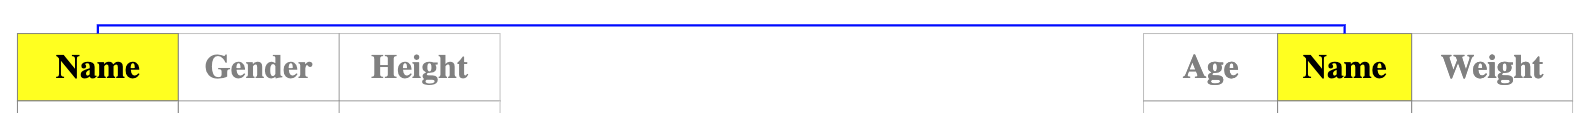
\includegraphics[scale = 0.25]{Masters-Thesis/img/keycol2.png}
    \caption{Key column step 2}
    \label{fig:keycol2}
\end{figure}

Then we need to show the users the structure of the joined table, to do this, we move all column headers except for the key from Table 2 to Table 1, this create new columns/variables in Table 1. After those elements have been moved over, the user can then see the basic structure of the resulted joined table because the rows below the new columns will be empty as shown in Fig.~\ref{fig:keycol3}. The next step is to fill in the empty parts of the rows.

\begin{figure}[H]
    % \centering
    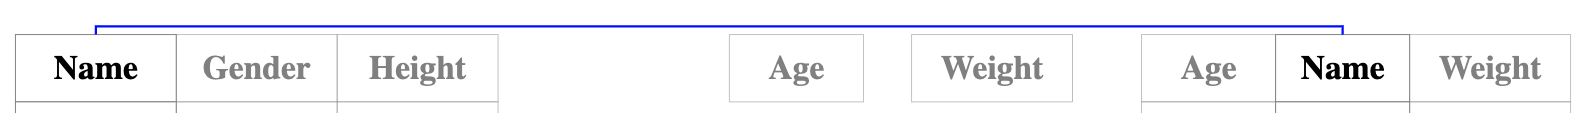
\includegraphics[scale = 0.25]{Masters-Thesis/img/keycol3.png}
    \caption{Key column step 3}
    \label{fig:keycol3}
\end{figure}

Once this structure has been emphasised the faded-out elements then revert back to normal. The original columns in table 1 will remain bold-ed whereas the new columns are not, this is to remind the user which columns are being joined on.

\begin{figure}[H]
    % \centering
    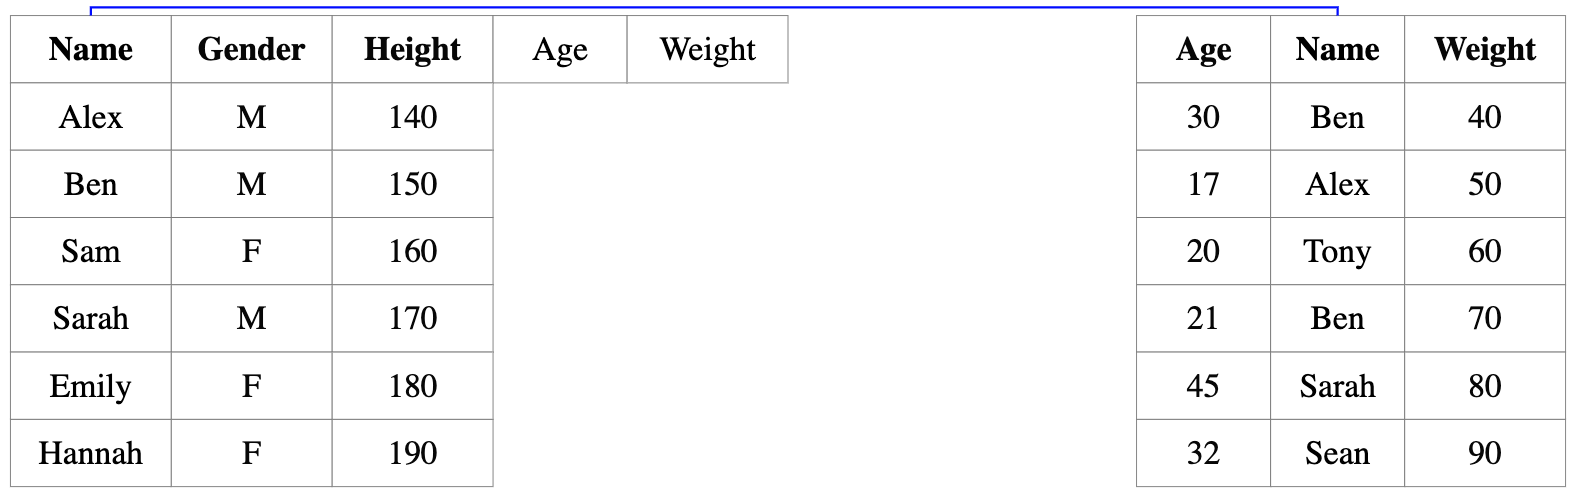
\includegraphics[scale = 0.25]{Masters-Thesis/img/keycol4.png}
    \caption{Key column step 4}
    \label{fig:keycol4}
\end{figure}

Next we will talk about how to fill in the empty rows, the joining process.

\section{Joining process}
In all joins, as part of joining information on rows from the two tables that belong together, elements from the key column in Table 1 will try find a match in the key column of table 2 sequentially until the end of Table 1.

\subsection{The case of a Single match}
Here, Alex is in the first row of Table 1. The join then tries to find Alex in table 2. 
In this scenario, there are matched elements from both key columns, since we have Alex in both tables, this means that these rows can be joined together. 

First, to draw attention to why and how these rows are being joined together, if there is a match on both tables, both matched elements from both key columns flash, and a line then links them together (Fig.~\ref{fig:single1}). 

\begin{figure}[H]
    % \centering
    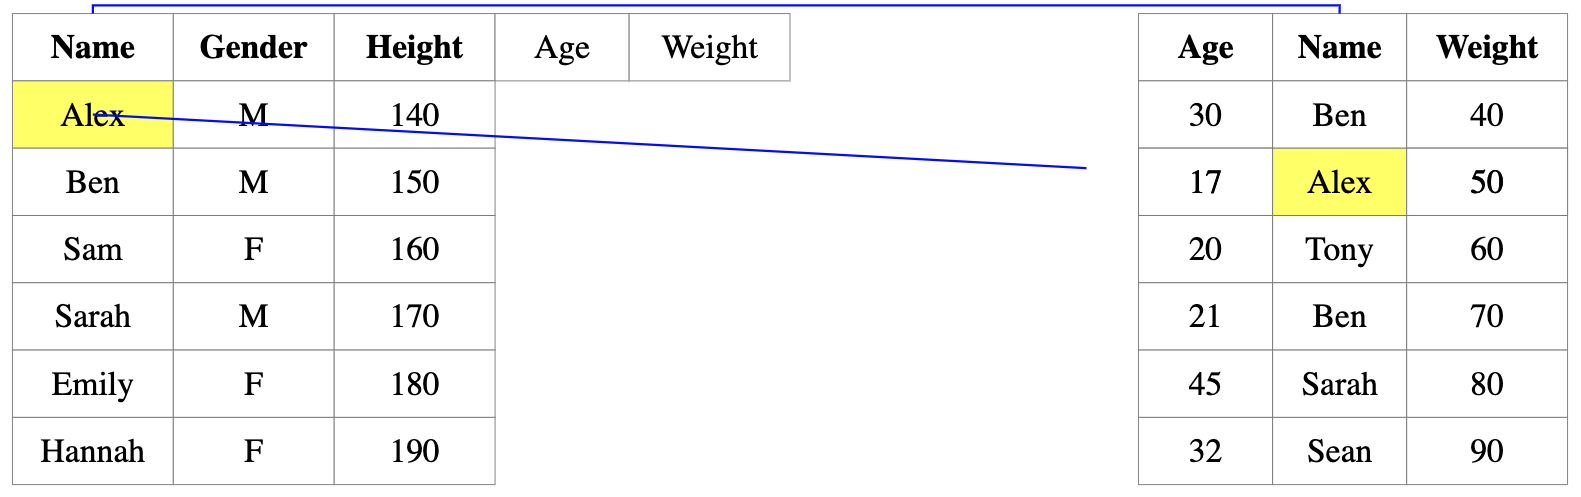
\includegraphics[scale = 0.25]{Masters-Thesis/img/single1.png}
    \caption{Single match step 1}
    \label{fig:single1}
\end{figure}

Second, a message will show explaining that we are currently “Matching Alex” (Fig.~\ref{fig:single2}).

\begin{figure}[H]
    % \centering
    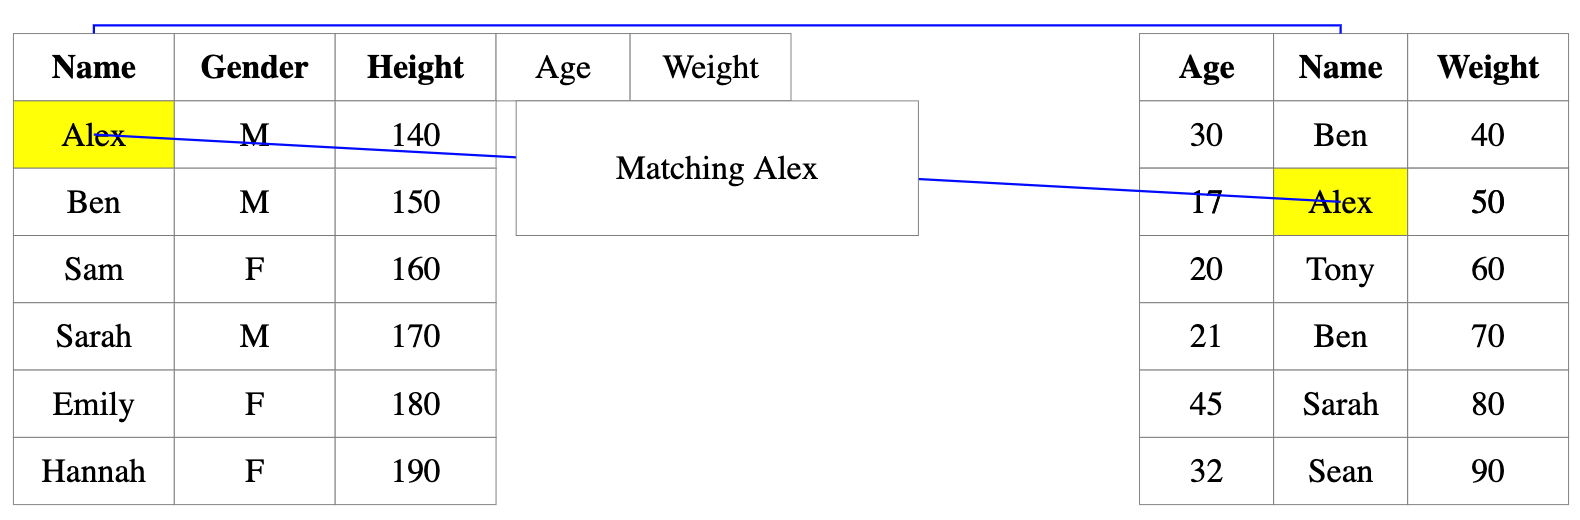
\includegraphics[scale = 0.25]{Masters-Thesis/img/single2.png}
    \caption{Single match step 2}
    \label{fig:single2}
\end{figure}

Then the actual join will perform, all elements except the key from the matched row in table 2 will move across to table 1 (Fig.~\ref{fig:single3} caught mid-move).

\begin{figure}[H]
    % \centering
    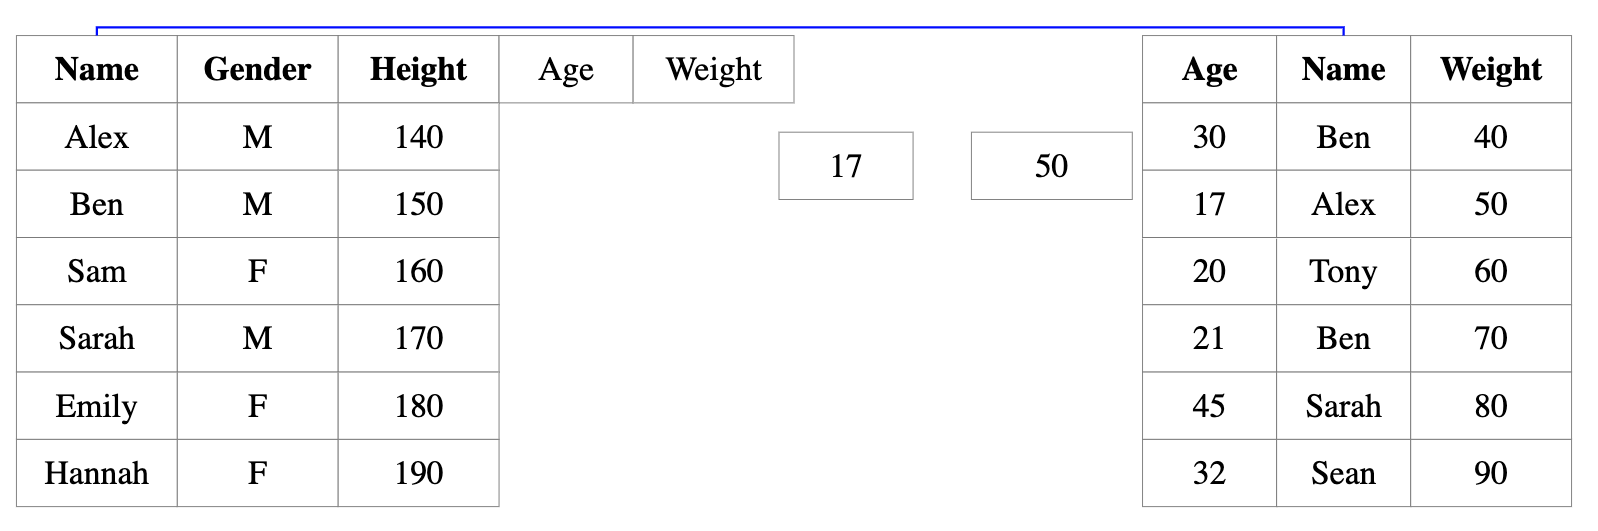
\includegraphics[scale = 0.25]{Masters-Thesis/img/single3.png}
    \caption{Single match step 3}
    \label{fig:single3}
\end{figure}

Lastly, to show the user that the information on Alex in Table 2 has now been used, and we don’t need to play attention to that particular row anymore, we fade out that particular row in Table 2 (Fig.~\ref{fig:single4}).

\begin{figure}[H]
    % \centering
    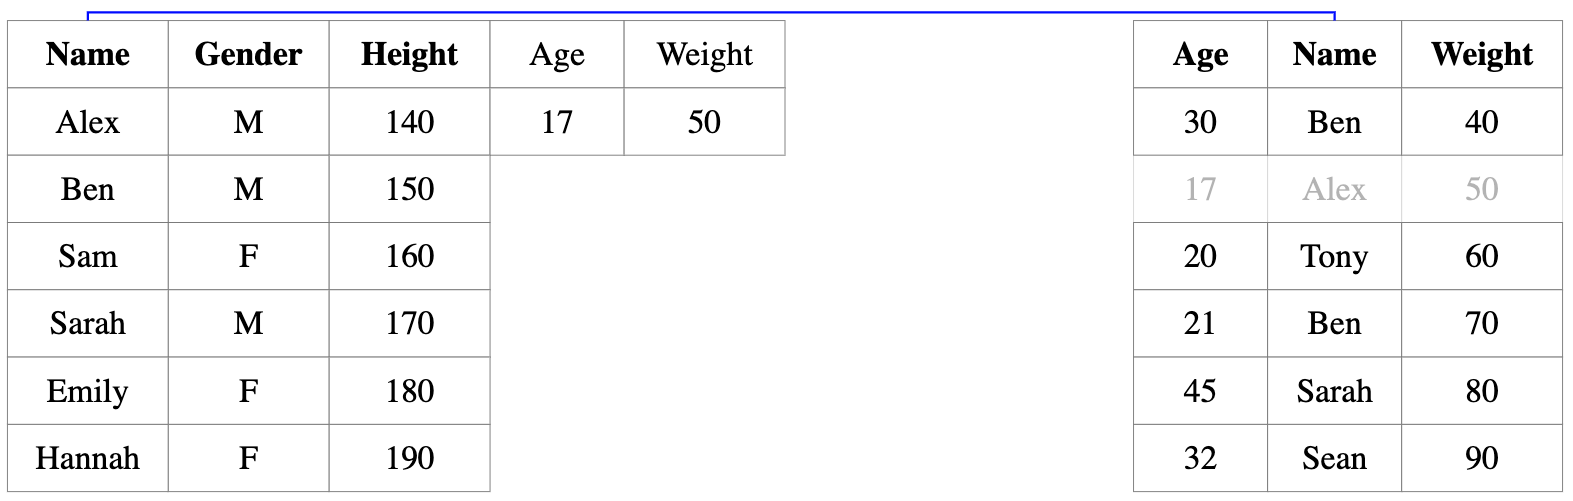
\includegraphics[scale = 0.25]{Masters-Thesis/img/single4.png}
    \caption{Single match step 4}
    \label{fig:single4}
\end{figure}

We then move on to Ben, then Sam and so on down Table 1.

\subsection{The case of Multiple matches}
This occurs when a row in Table 1 matches multiple rows in Table 2.

Like the single match scenario, to allow the users focus on the rows that are being matched, their elements will flash, but this time we will see that there is more than one line matching the rows because there is more than one match found. \\

To reinforce the user that there are more than one rows that match and we want to draw attention to some different behaviour, we show “2 matches found for Ben” (Fig.~\ref{fig:multiple1}).

\begin{figure}[H]
    % \centering
    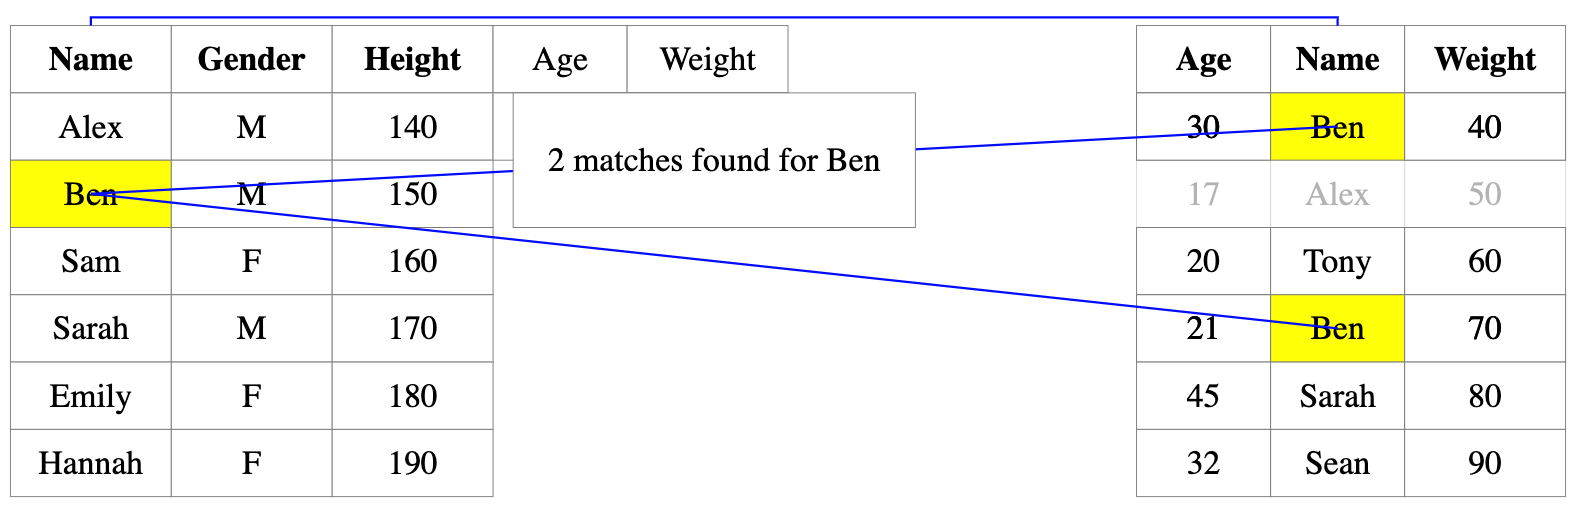
\includegraphics[scale = 0.25]{Masters-Thesis/img/multiple1.png}
    \caption{Multiple matches step 1}
    \label{fig:multiple1}
\end{figure}

We want to move two rows of data from Table 2 across to Table 1 This causes a problem, because there is only one row in Table 1 which matched Table 2.  \\

To solve this we need to compensate by adding an extra row to Table 1, duplicating the matched row from Table 1 (Fig.~\ref{fig:multiple2}). Fig.~\ref{fig:multiple2} also shows the two "Ben" rows from Table 2 in the process of being moved across.  

\begin{figure}[H]
    % \centering
    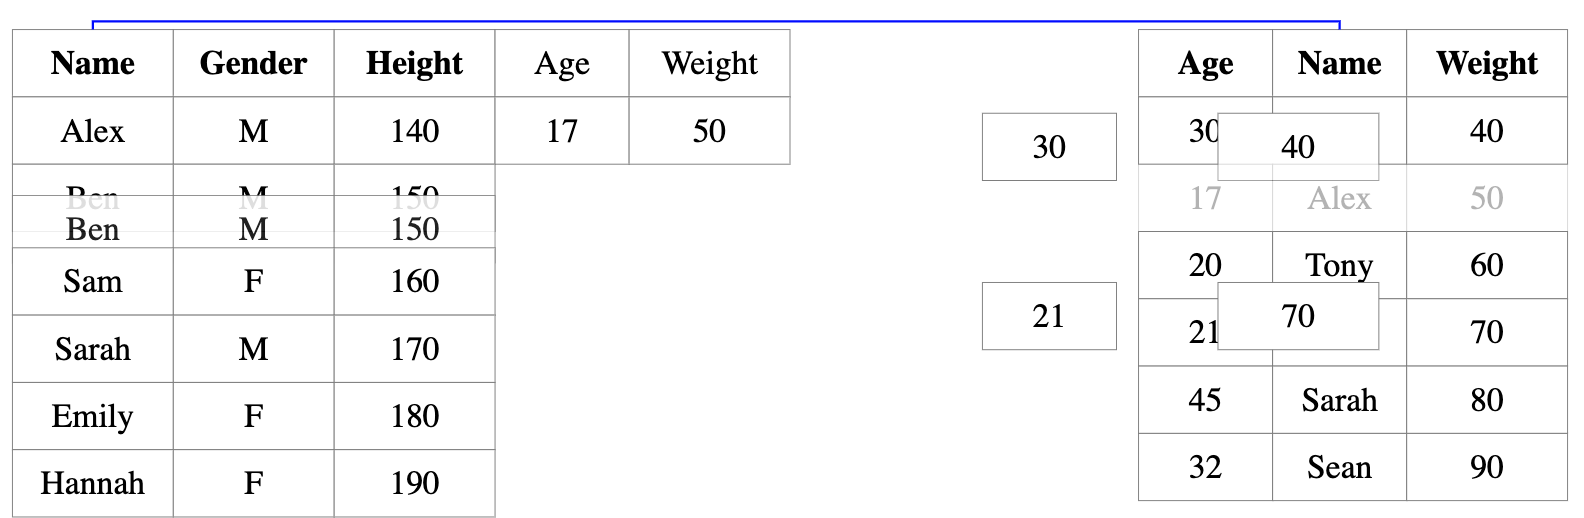
\includegraphics[scale = 0.25]{Masters-Thesis/img/multiple2.png}
    \caption{Multiple matches step 2}
    \label{fig:multiple2}
\end{figure}

\subsection{The case of No match}
What happens when we get to a row in Table 1 with no match in Table 2? Here we don’t have Sam in the key column of Table 2 (Fig.~\ref{fig:nomatch1}). \\

To show this we first flash the row that is currently looking for a match to show the user that this row is currently looking for a match. 
Second, we animate a line to move from that particular element towards Table 2 to show that the join is in the process of looking for a match. 
Third, we stop the line from moving towards table 2 and a pop up question mark. 
Lastly, we pop up a message telling the user that there were no match found. \\

Actions for the no-matches found . case differs between different type of join, as discussed in in paragraphs that follow.

\begin{figure}[H]
    % \centering
    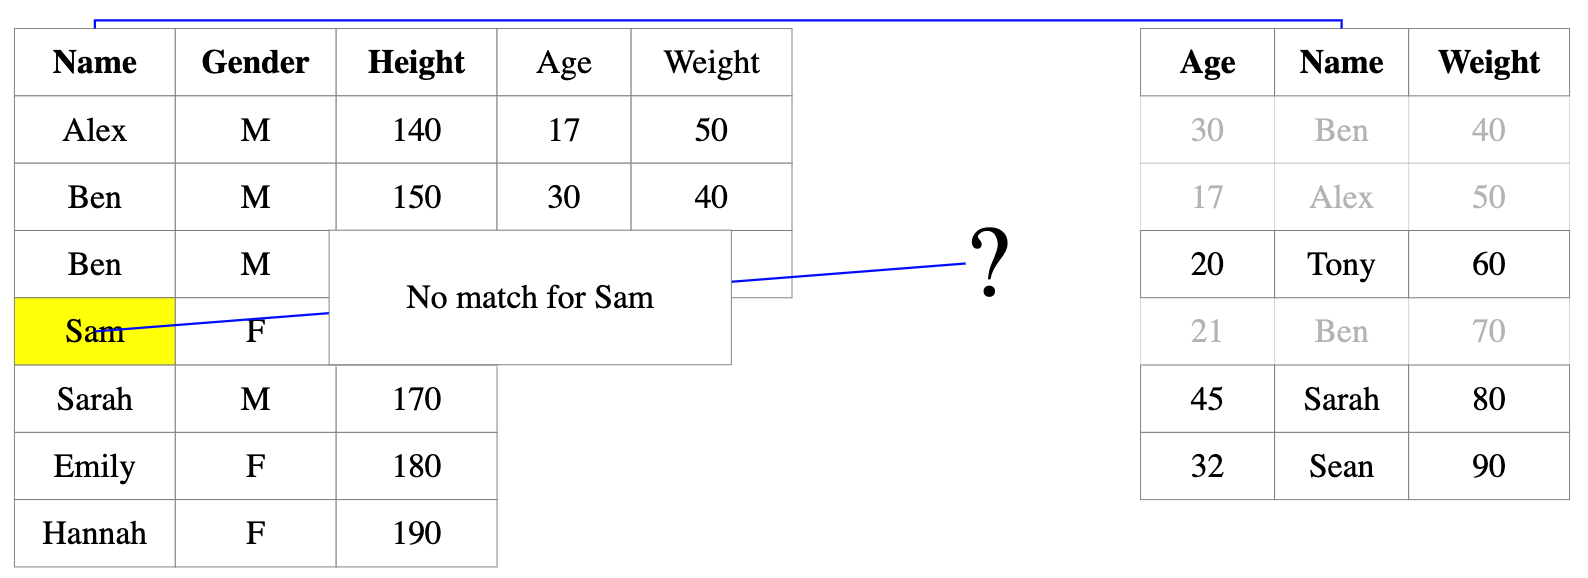
\includegraphics[scale = 0.25]{Masters-Thesis/img/nomatch1.png}
    \caption{No match}
    \label{fig:nomatch1}
\end{figure}

\section{Left/Right Join}
We only show a left join because we get the same resulting join as a right join by left-joining in the reverse order. \textit{Left/Right joins} are also known as \textit{left/right outer joins}.

\begin{figure}[H]
    \centering
    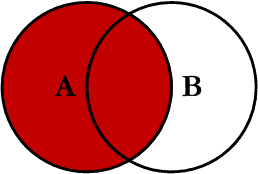
\includegraphics[scale = 0.5]{Masters-Thesis/img/vennleft.png}
    \caption{Venn diagram of Left Join}
    \label{fig:vennleft}
\end{figure}

The definition of a left join is that it returns  data relating to all rows from Table 1, and the matching rows from Table 2. 

For a left join, when there are no matches found, the row in Table 1 is still kept, but there is no information on Table 2 variables for this unit. Therefore those values from the new Table 2 variables are missing (NA).
To show this we then replace the missing values with NA which is the term for missing value in R. Since Sam was not found in Table 2, we fill their Age and Weight columns with NA.

\begin{figure}[H]
    % \centering
    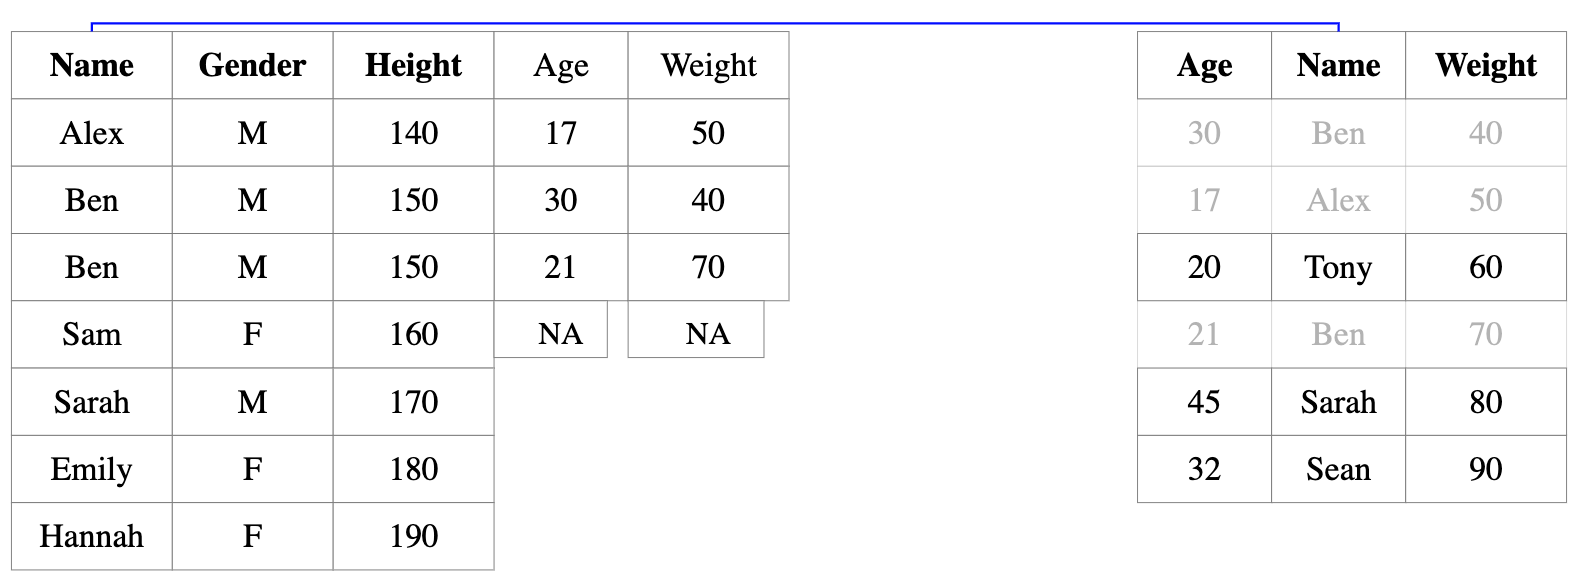
\includegraphics[scale = 0.25]{Masters-Thesis/img/left1.png}
    \caption{Left Join step 1}
    \label{fig:left1}
\end{figure}

After the last row in Table 1 finishes matching, the join is complete. To show the user which rows were used, we can see that some rows are faded out in Table 2. By this strategy, all the usable information in Table 2 has already been used. What is left in Table 2 corresponds to units that are not to be used because they do not appear in Table 1 (see Fig.~\ref{fig:left2}).

\begin{figure}[H]
    \centering
    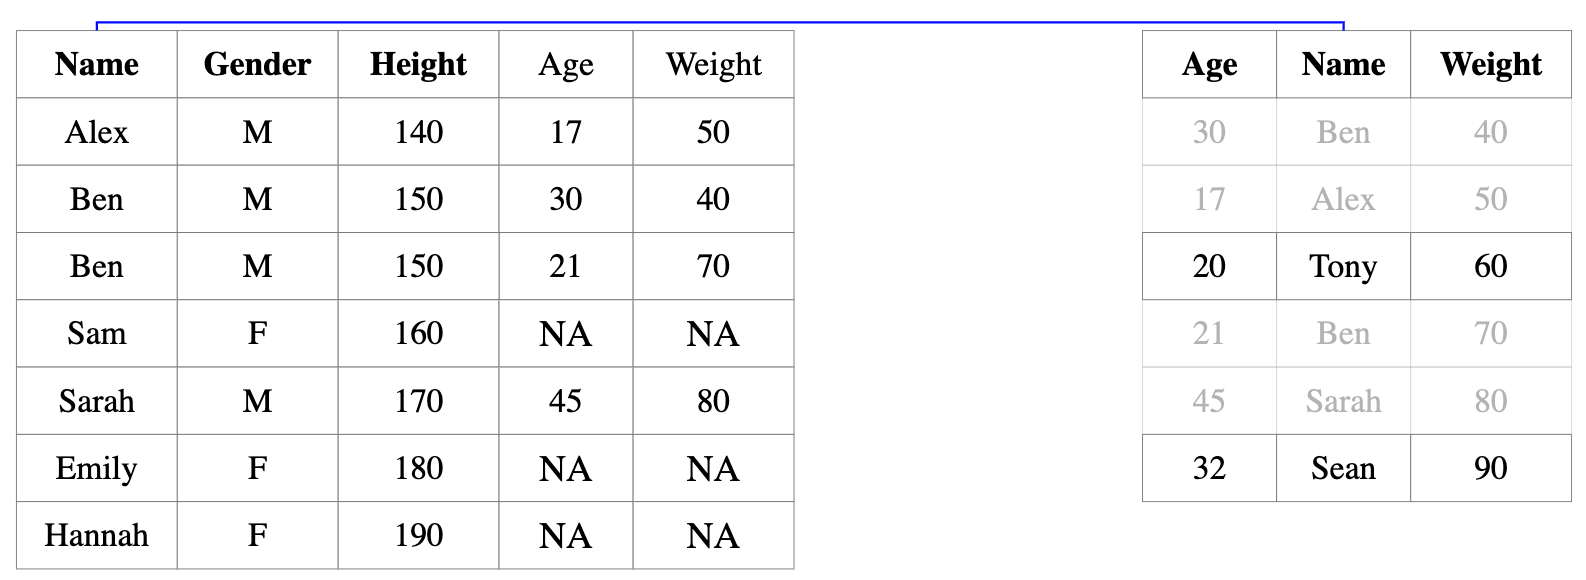
\includegraphics[scale = 0.25]{Masters-Thesis/img/left2.png}
    \caption{Left Join step 2}
    \label{fig:left2}
\end{figure}

To show the user that the join is complete, Table 2 fade away because it is not needed anymore, and Table 1 is moved to the middle so the user can see clearly the resulted joined Table (Fig.~\ref{fig:left3}). 

\begin{figure}[H]
    \centering
    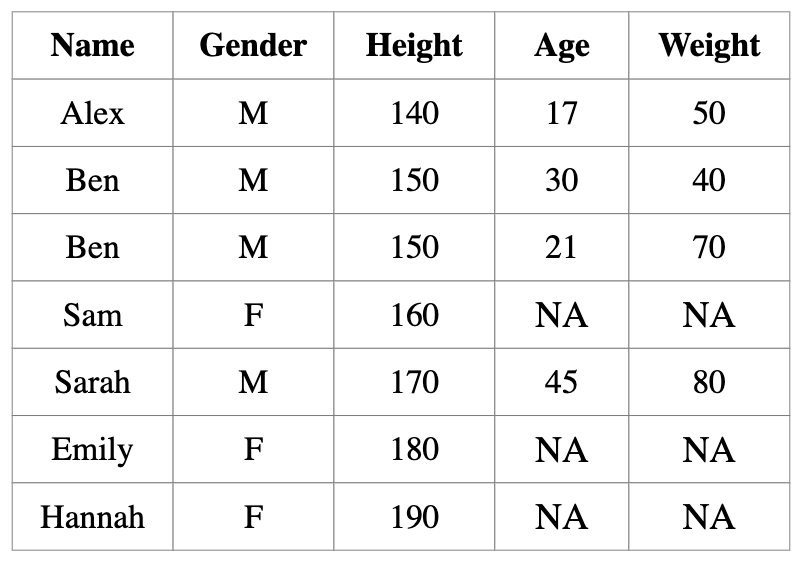
\includegraphics[scale = 0.25]{Masters-Thesis/img/left3.png}
    \caption{Left Join step 3}
    \label{fig:left3}
\end{figure}

\section{Inner Join}
The main idea of a inner join is to combine information on only those units that appear in \textbf{both} Table 1 and Table 2. That is why they are typically represented by a intersection in a Venn diagram. 

\begin{figure}[H]
    \centering
    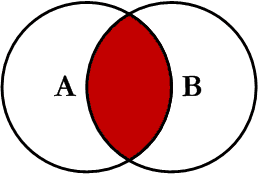
\includegraphics[scale = 0.5]{Masters-Thesis/img/venninner.png}
    \caption{Venn diagram of Inner Join}
    \label{fig:venninner}
\end{figure}

The definition of a inner join is it returns rows that have matching key column values in both tables. This is similar to the left join explained above but since it only returns rows that have matching key columns in both tables. When no match is found for a Table 1 row in Table 2, we remove that row in Table 1 instead of filling in NA for the missing values (Fig.~\ref{fig:inner1}, \ref{fig:inner2}). 

\begin{figure}[H]
    % \centering
    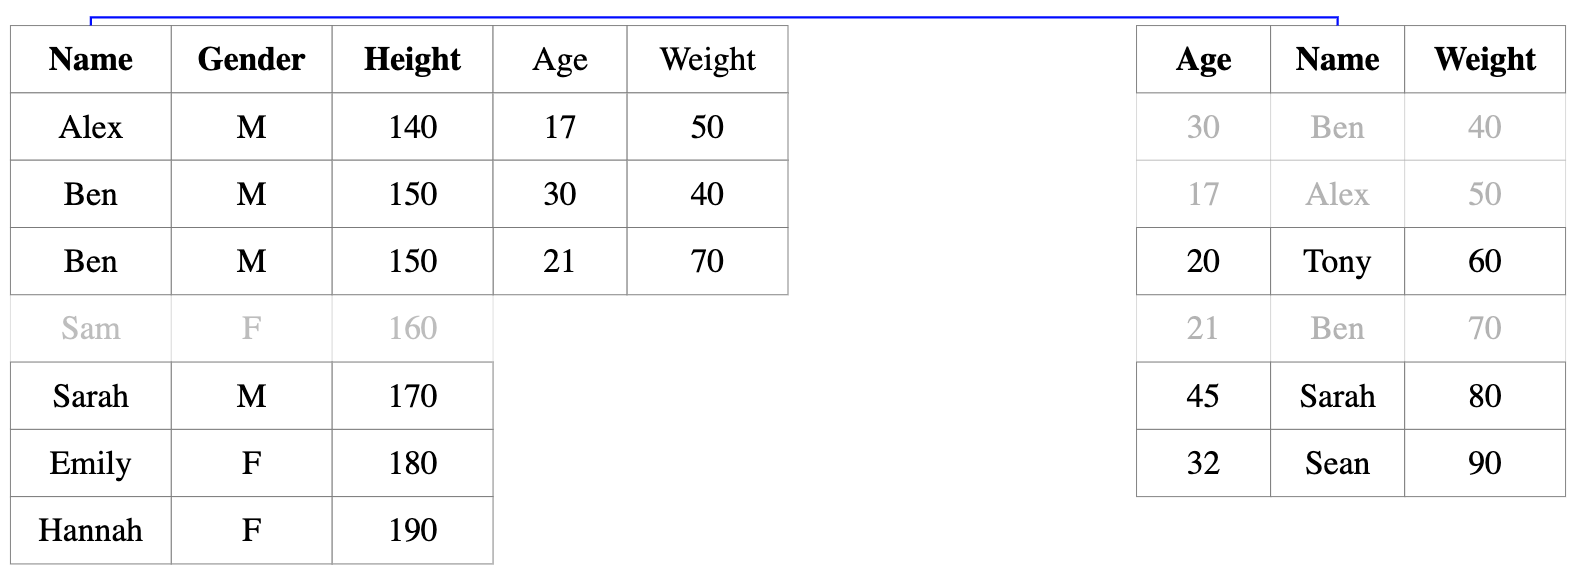
\includegraphics[scale = 0.25]{Masters-Thesis/img/inner1.png}
    \caption{Inner Join step 1}
    \label{fig:inner1}
\end{figure}

At the end of the join, the user will be able to see which rows did not find a match, from the gaps between rows in Table 1. This is to remind the user that there are rows that were removed because there were no matches for them.

\begin{figure}[H]
    % \centering
    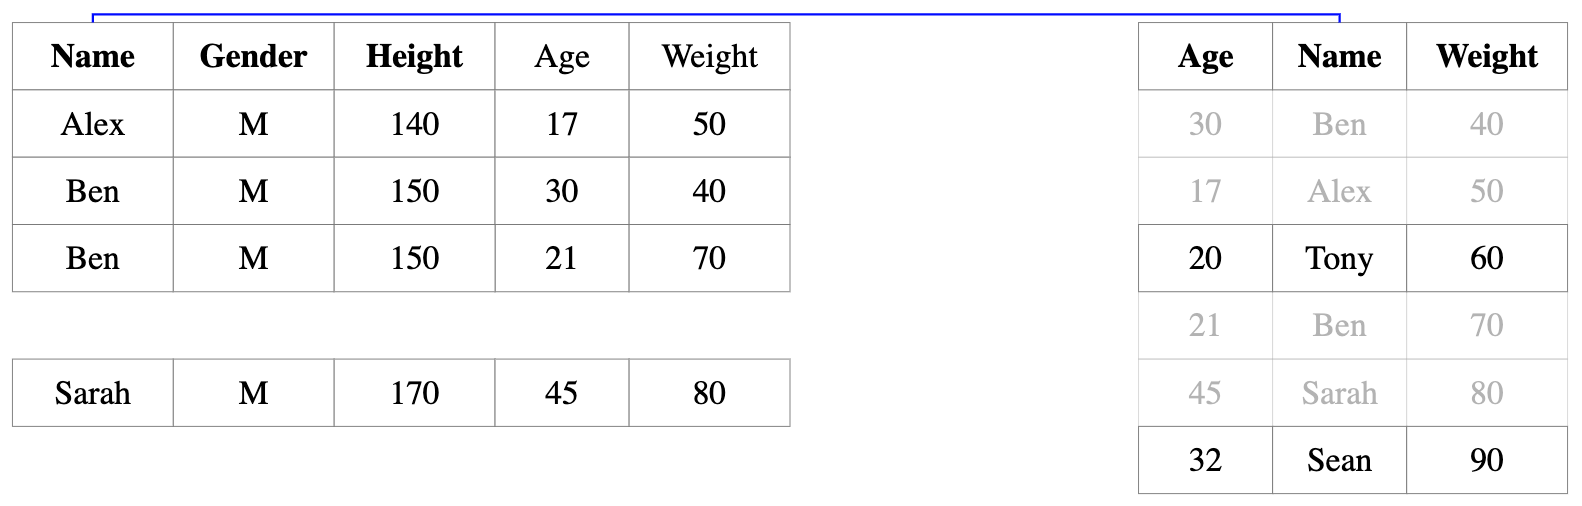
\includegraphics[scale = 0.25]{Masters-Thesis/img/inner2.png}
    \caption{Inner Join step 2}
    \label{fig:inner2}
\end{figure}

Similar to left join, to show that the join is finished, Table 2 will be removed and the resulted joined table will be centred. The only difference is that all the rows will be pushed together to fill in the gaps produced by the removed rows (Fig.~\ref{fig:inner3}).

\begin{figure}[H]
    \centering
    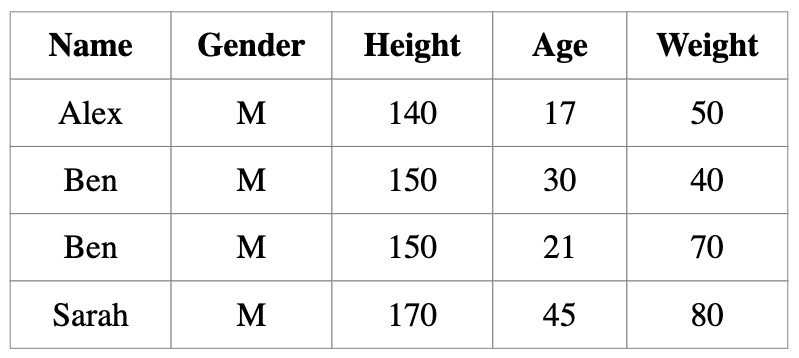
\includegraphics[scale = 0.3]{Masters-Thesis/img/inner3.png}
    \caption{Inner Join step 3}
    \label{fig:inner3}
\end{figure}

\section{Full Join}
The full join is also known as a complete join. The main idea of a full join is to combine information on all units that appear in either Table 1 or Table 2 or both. That is why they are often represented by a union in a Venn diagram.

\begin{figure}[H]
    \centering
    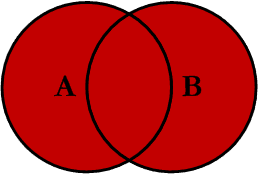
\includegraphics[scale = 0.5]{Masters-Thesis/img/vennfull.png}
    \caption{Venn diagram of Full Join}
    \label{fig:vennfull}
\end{figure}

The definition of a full join is it returns all rows relating to key column values found in Table 1, Table 2 or both. For a complete join, the first step of the joining process is the same as a left join. The difference is that when the matching process is done, the left join is complete, whereas the full join now will move the unmatched rows from the Table 2 to Table 1. \\

The problem here is that we will need to move the remaining unmatched rows from Table 2 that have not been used, these are rows in Table 2 that are not faded out (because they have already been used). 

First, to catch the users attention, we flash the elements from the key column in the unmatched rows in Table 2.
Second, we animate a line and a question mark showing the user that they are the unmatched rows and there is no where for them to go (Fig.~\ref{fig:full1}).

\begin{figure}[H]
    % \centering
    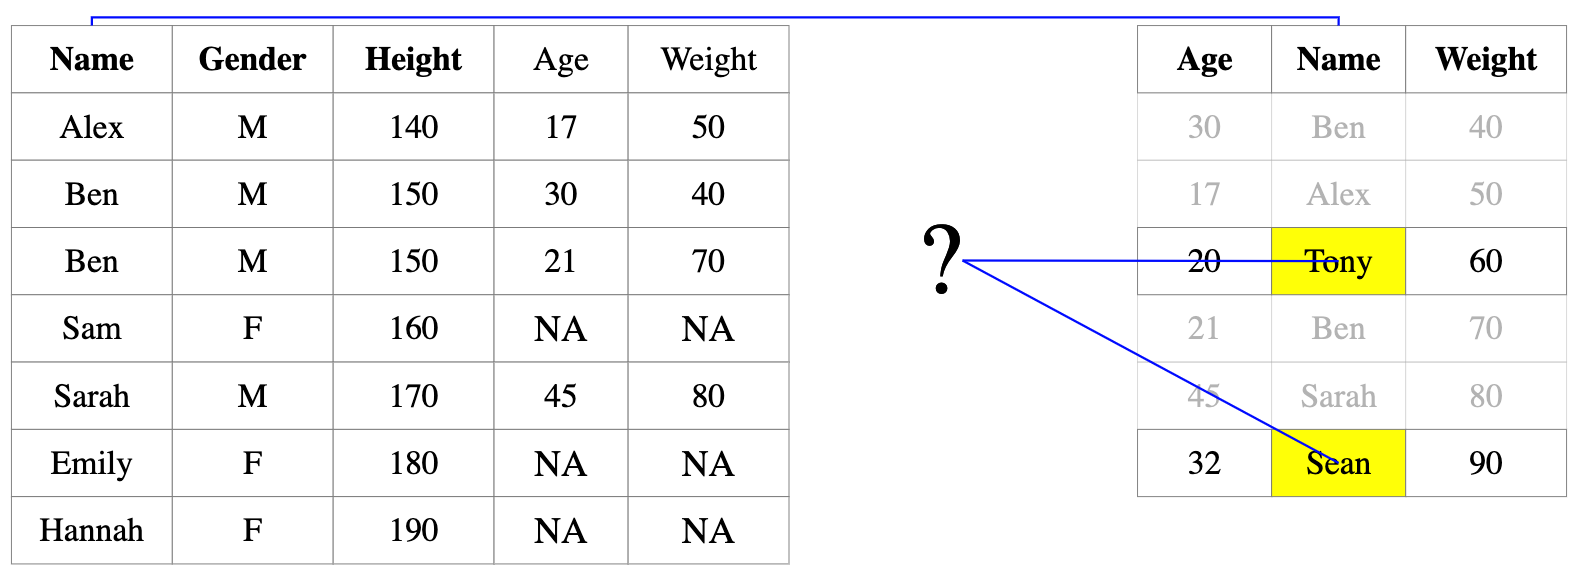
\includegraphics[scale = 0.25]{Masters-Thesis/img/full1.png}
    \caption{Full Join step 1}
    \label{fig:full1}
\end{figure}

\newpage
Third, we show a message indicating that (Fig.~\ref{fig:full2}). Then we move the unused rows across to Table 1, this is to remind the user what the next step is.

\begin{figure}[H]
    % \centering
    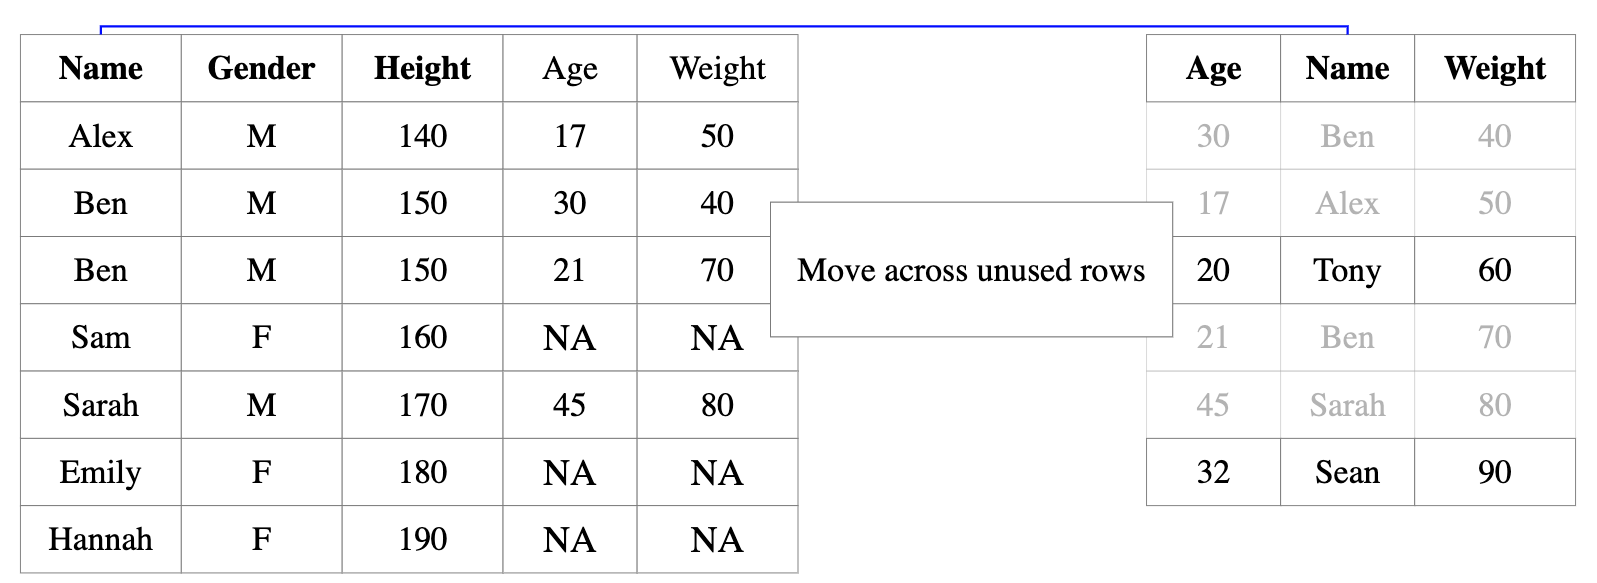
\includegraphics[scale = 0.25]{Masters-Thesis/img/full2.png}
    \caption{Full Join step 2}
    \label{fig:full2}
\end{figure}

Fourth, we move the unmatched rows from Table 2 across to Table 1, to their corresponding column in row order (Fig.~\ref{fig:full3}).

\begin{figure}[H]
    % \centering
    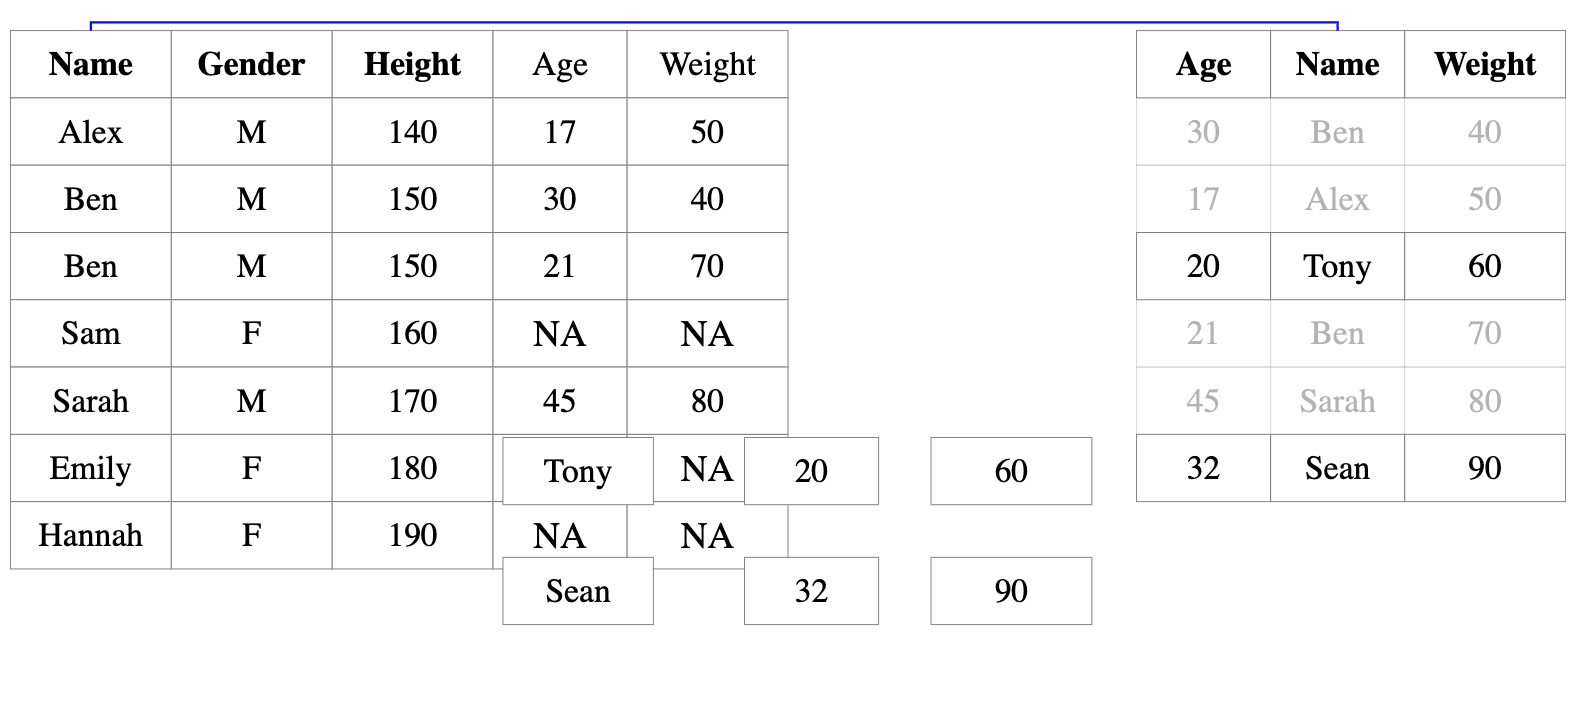
\includegraphics[scale = 0.25]{Masters-Thesis/img/full3.png}
    \caption{Full Join step 3}
    \label{fig:full3}
\end{figure}

\newpage

After the rows are moved across, the cells corresponding to the Table 1 variables will be empty. To complete the join we will need to fill these with NAs to indicate that these are missing values. \\

Therefore, fifth, to convey this idea, we flash this region in red, question marks will also appear showing the user that this region is missing, and that we do not have any information in these data (Fig.~\ref{fig:full4}). 

\begin{figure}[H]
    % \centering
    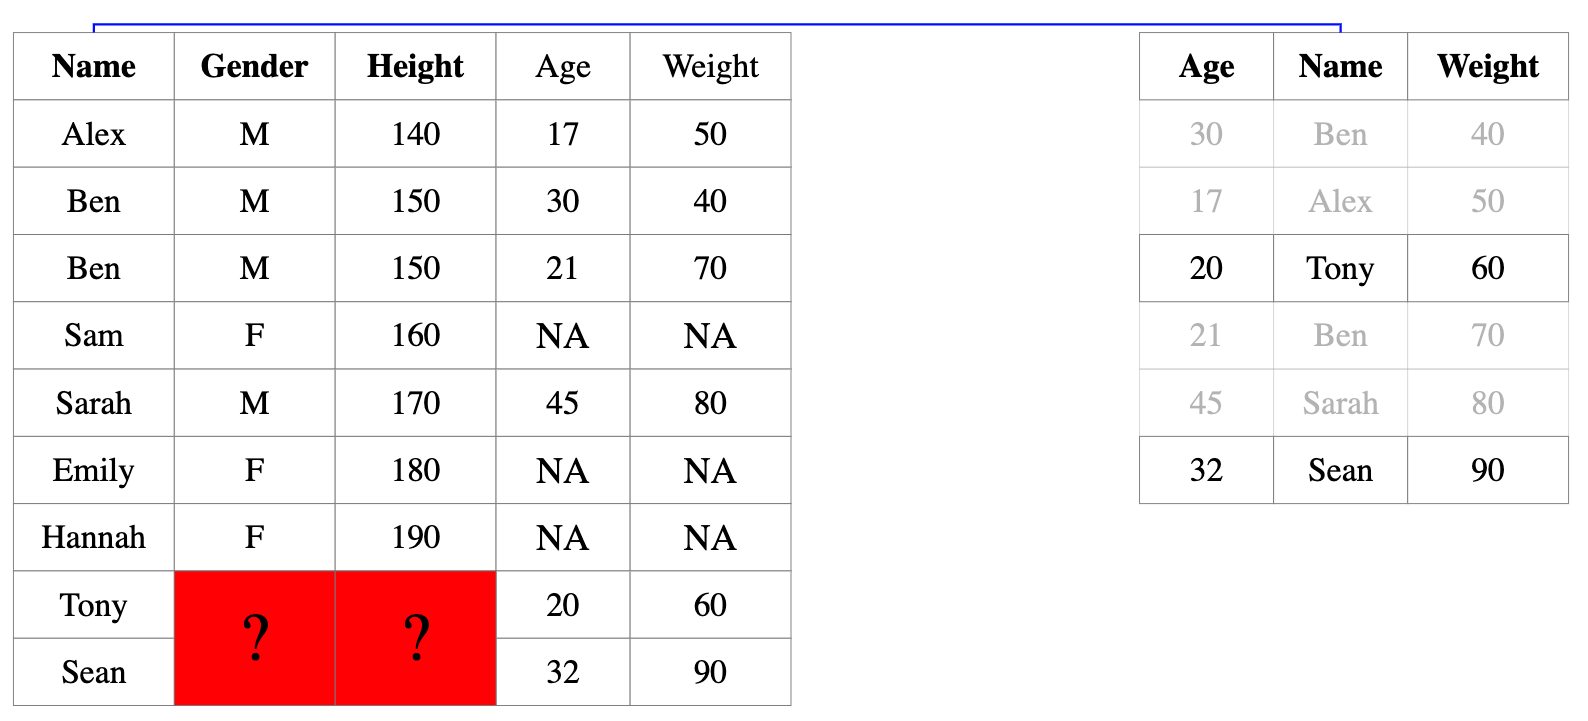
\includegraphics[scale = 0.25]{Masters-Thesis/img/full4.png}
    \caption{Full Join step 4}
    \label{fig:full4}
\end{figure}

Then we replace these empty elements with NA, similar to what we did with a left join (Fig.~\ref{fig:full5}). 

\begin{figure}[H]
    % \centering
    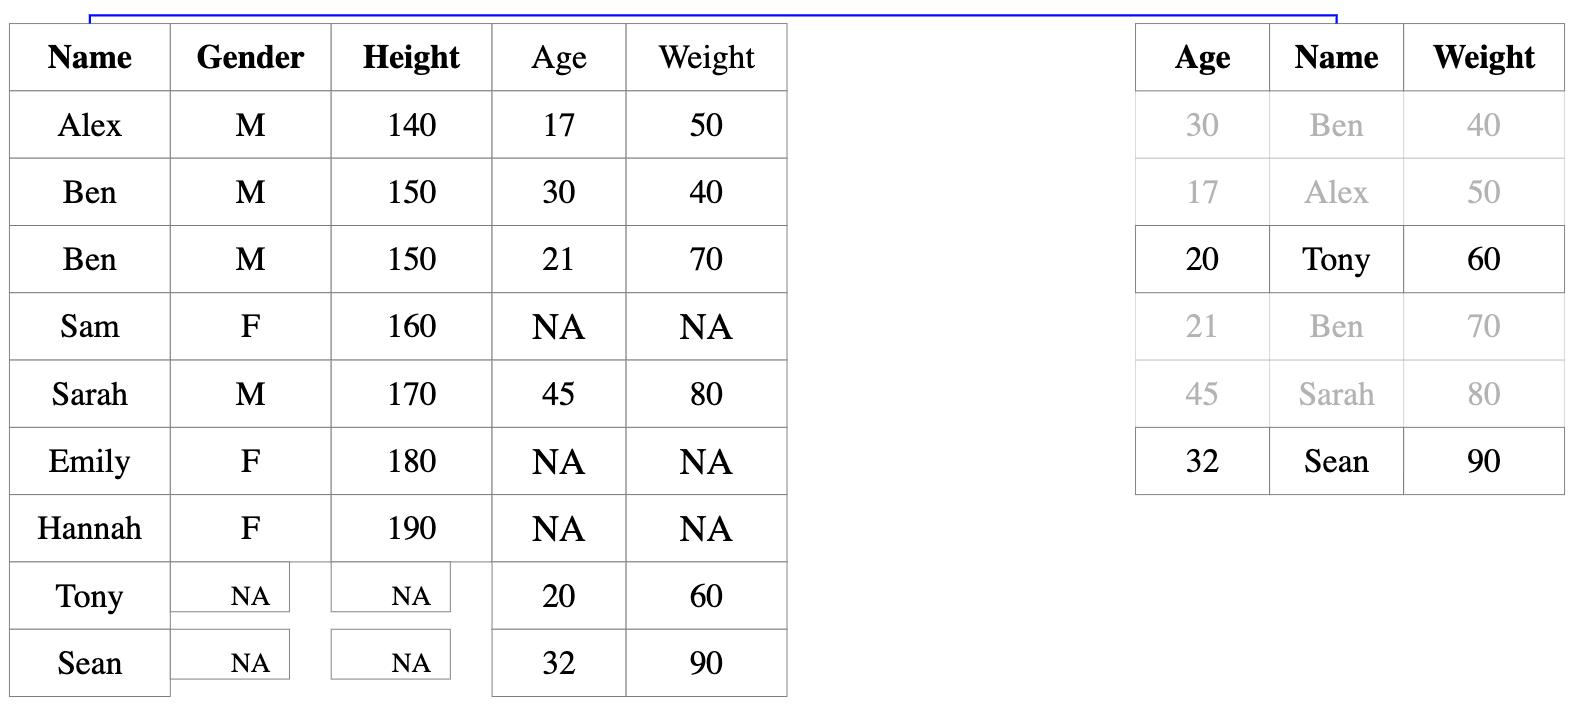
\includegraphics[scale = 0.25]{Masters-Thesis/img/full5.png}
    \caption{Full Join step 5}
    \label{fig:full5}
\end{figure}

\newpage

Lastly, at the end of the join, we isolate the resulted joined table to the middle to show the user that this is finished (Fig.~\ref{fig:full6}).

\begin{figure}[H]
    \centering
    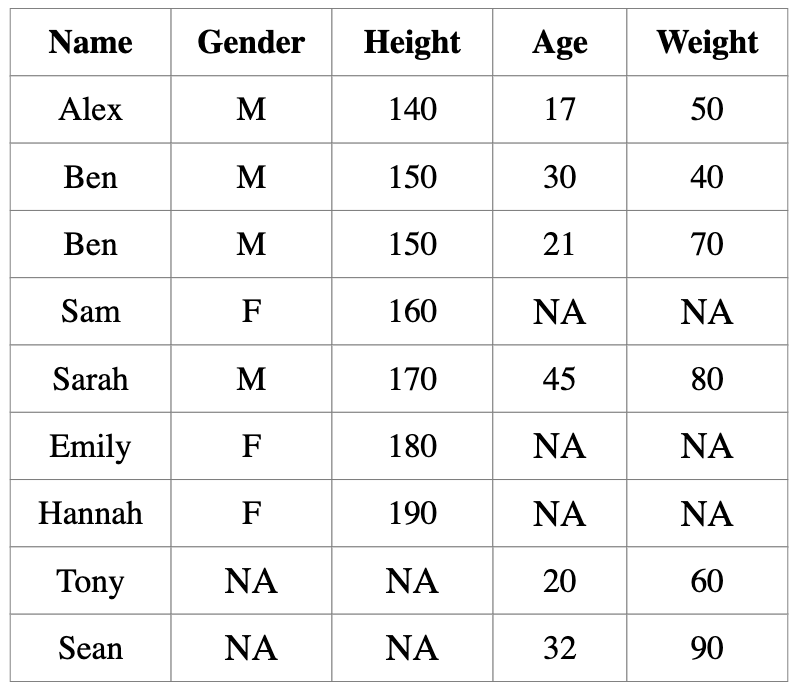
\includegraphics[scale = 0.3]{Masters-Thesis/img/full6.png}
    \caption{Full Join step 6}
    \label{fig:full6}
\end{figure}
